% --------------------------------------------------------------------------
% Template for Project Course paper; to be used with:
%          ProjectCourse21.sty  - Project Course 2021 LaTeX style file, and
%
% --------------------------------------------------------------------------

\documentclass{article}
\usepackage{MAECapstoneCourse,amsmath,graphicx,url,times}
\usepackage{color}
\usepackage[utf8]{inputenc}
\pagenumbering{arabic}

% Example definitions.
% --------------------
\def\defeqn{\stackrel{\triangle}{=}}
\newcommand{\symvec}[1]{{\mbox{\boldmath $#1$}}}
\newcommand{\symmat}[1]{{\mbox{\boldmath $#1$}}}

% Title.
% --------------------
\title{Sound Event Classification}

% PUT NAMES IN ALPHABETIC ORDER (consider surname first)
\name{Chiara Auriemma, Francesca Benesso, Anna Fusari, Filippo Marri}
\address{Dipartimento di Elettronica, Informazione e Bioingegneria (DEIB), Politecnico di Milano\\
Piazza Leonardo Da Vinci 32, 20122 Milano, Italy\\   
\tt{[chiara.auriemma,francesca1.benesso]@mail.polimi.it}\\
\tt{[anna.fusari,filippo.marri]@mail.polimi.it}
}

\begin{document}

\ninept
\maketitle

\begin{sloppy}

\begin{abstract}
  Sound Event Classification (SED) has become an important task in the field of
  audio processing, with applications ranging from environmental monitoring to
  human-computer interaction. Aim of this project is to develop a sound event classification system
  based on a Convolutional Recurrent Neural Network (CRNN) architecture training it on the ESC-50 dataset.
  At the end, the performances of the model are compared with the ones of a state-of-the-art model (QUALE?).
\end{abstract}

\begin{keywords}
Sound Event Classification, Convolutional Recurrent Neural Network
\end{keywords}

\section{Introduction}
\label{sec:intro}
Sound Event Classification (SED) is a task that involves the identification and classification of
specific sound events within an audio signal. This task has gained significant attention in recent years
due to its wide range of applications, including environmental monitoring\cite{birdsCNN2017}, human-computer interaction\cite{emotionRecognition2021}, and multimedia content analysis\cite{kumar2016weaklysupervisedscalableaudio}.
The goal of SED is to accurately detect and classify sound events in real-time or from pre-recorded audio data.
The process of SED typically involves several steps, including feature extraction, model training, and evaluation\cite{ReviewSoundEvent2025}.
Commonly used features include Mel-frequency cepstral coefficients (MFCCs), spectrograms, and log-mel spectrograms.
Model training involves using labeled audio data to train a machine learning model to recognize and classify sound events.
Various machine learning algorithms can be used for SED, including support vector machines (SVMs), decision trees, and deep
learning models such as convolutional neural networks (CNNs) and recurrent neural networks (RNNs)\cite{DescriptiveESC2022}.
The choice of algorithm depends on the complexity of the task and the available data.
Evaluation of the SED system is typically done using standard metrics such as accuracy, precision, recall, and F1-score.

\section{Dataset analysis and preprocessing}
\label{sec:format}

The dataset used for this project is the well-known ESC-50 dataset \cite{piczak2015dataset}, which contains
2000 labeled sound events from 50 different classes, with each class containing 40 samples. Each song of the dataset is available in WAV format with
a sample rate of 44.1 kHz and a bit depth of 16 bits.

\subsection{Dataset analysis}
According to the analysis that will be done on the results inspired by (CHIEDERE ARTICOLOOOO), the type of soound events in the dataset can be divided into three main categories:
\begin{itemize}
    \item \textbf{Transient sounds}: This category includes sounds that have a short duration and are characterized by a sudden onset, such as a dog barking, a door slamming, or a gunshot.
    \item \textbf{Continous sounds}: This category includes sounds that have a longer duration and are characterized by a continuous or sustained sound, such as a car engine running, a train passing, or a river flowing.
    \item \textbf{Intermittent sounds}: This category includes sounds that have a periodic or irregular pattern, such as a clock ticking, a bird chirping, or a phone ringing.
\end{itemize}

According to what is reported in the paper in which the ESC-50 dataset is presented \cite{piczak2015dataset}, we higlight how some sounds are more difficult to classify than others,
such as the sounds of a washing machine, an helicopter, or an engine due to their similar spectrograms.
This happens not only for machines, but for humans too. This will be taken into account in the results section, where we will see how the model performs on different classes of sounds.

It is also important to note that, even though we consider the same class, the variability of the sounds is very high, as we can see by comparing the spectrograms of three different
samples of the \textit{dog barking} class.

Furthermore, we underline how some of the ambiental sounds, like the one of the wind, have no univoque structure: by breaking down (phrasl verb...)
their spectrograms in their harmonic and percussive components, it is evident that the difference it is not so clear since the two plots are almost equal.

\subsection{Dataset preprocessing}
Drawing inspiration by the Salamon and Bello paper\cite{salamon2017deep}, five different techniques have been implemented to process the dataset:
\begin{itemize}
    \item \textbf{Time Stretching (TS)}: the audio signal is stretched or compressed in time by a random factor within a specified range.
    \item \textbf{Pitch Shifting (PS)}: the audio signal is shifted in pitch by a random factor within a specified range.
    \item \textbf{Background Noise (BN)}: a Gaussian noise is added to the audio signal with a specified SNR range and activation probability.
    \item \textbf{Dynamic Range Compression (DRC)}: the dynamic range of the audio signal is compressed.
    \item \textbf{Convolution with Impulse Responses (CIR)}: the audio signal is convolved with the \textit{MIT Acoustical Reverberation Scene Statistics Survey} dataset of impulse responses\cite{traer2016statistics} to simulate different acoustic environments. This time again, an activation probability is used to increase variability.
\end{itemize}



\section{Feature Extraction and Cross-Validation}
\textit{La luna vide dal cielo}
\\\textit{Rosita baciar Manuelo}
\\\textit{Con tanto languor, con tanto ardor}
\\\textit{Che s'ammantò d'un velo}

\label{sec:pagelimit}

You are allowed a total of 5 pages for your document. Up to 4 pages may 
contain technical content, figures, and references, while the 5th page 
may contain only references. This is the max-imum number of pages that 
will be accepted, including all figures, tables, and references. Any 
documents that exceed the 5-page limit will be rejected. Any documents 
with a 5th page containing anything other than references will be rejected.


\section{PAGE TITLE SECTION}
\label{sec:pagestyle}

The paper title (on the first page) should begin 0.98 inches 
(25 mm) from the top edge of the page, centered, completely 
capitalized, and in Times 14-point, boldface type.  
The authors' name(s) and affiliation(s) appear below the title
in capital and lower case letters.  Papers with multiple authors 
and affiliations may require two or more lines for this information.

\section{TYPE-STYLE AND FONTS}
\label{sec:typestyle}


In nine point type font, capital letters are 2 mm high.  
{\bf If you use the smallest point size, there should be 
no more than 3.2 lines/cm (8 lines/inch) vertically.}  
This is a minimum spacing; 2.75 lines/cm (7 lines/inch) 
will make the paper much more readable. Larger type sizes 
require correspondingly larger vertical spacing. Please do 
not double-space your paper. True-Type 1 fonts are preferred.

The first paragraph in each section should not be indented, 
but all the following paragraphs within the section should 
be indented as these paragraphs demonstrate.

\section{SECTION TITLE}
\label{sec:majhead}

Major headings, for example, ``1. Introduction'', should 
appear in all capital letters, bold face if possible, 
centered in the column, with one blank line before, 
and one blank line after. Use a period (``.'') after 
the heading number, not a colon.

\subsection{Subsection Title}
\label{ssec:subhead}

Subheadings should appear in lower case (initial word 
capitalized) in boldface. They should start at the left 
margin on a separate line. 
 
\subsubsection{Sub-subsection Title}
\label{sssec:subsubhead}

Sub-subheadings, as in this paragraph, are discouraged. 
However, if you must use them, they should appear in 
lower case (initial word capitalized) and start at the 
left margin on a separate line, with paragraph
text beginning on the following line. They should be 
in italics. 
 

\section{ILLUSTRATIONS, GRAPHS, AND PHOTOGRAPHS}
\label{sec:illust}

Illustrations must appear within the designated margins.  
They may span the two columns. If possible, position 
illustrations at the top of columns, rather than in 
the middle or at the bottom. Caption and number every 
illustration. All halftone illustrations must be clear 
black and white prints. Colors may be used, but they 
should be selected so as to be readable when printed 
on a black-only printer.

Since there are many ways, often incompatible, of 
including images (e.g., with experimental results) 
in a \LaTeX\ document, an example of how to do
this is presented in Fig.~\ref{fig:results}.

% Below is an example of how to insert images. 
% -------------------------------------------------------------------------
\begin{figure}[t]
  \centering
  \centerline{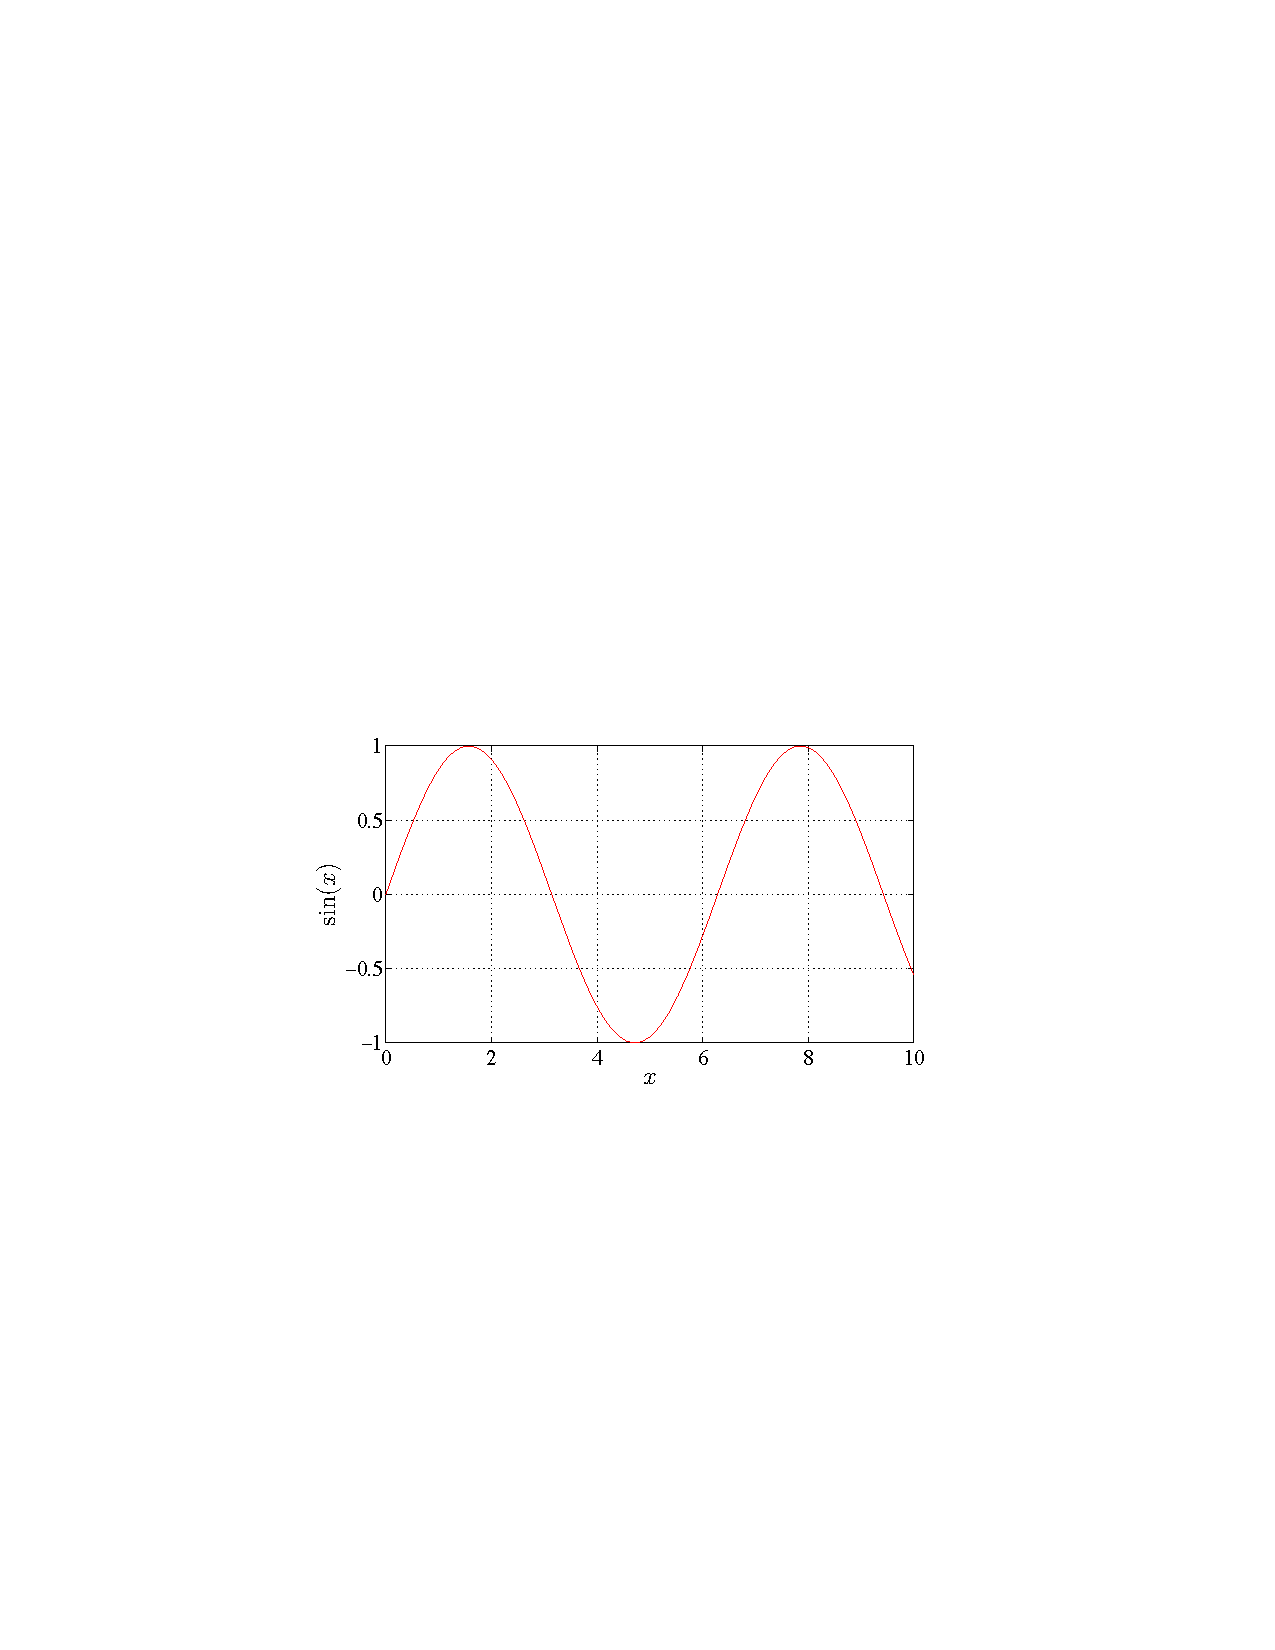
\includegraphics[width=\columnwidth]{fig1a}}
  \caption{Example of a figure with experimental results.}
  \label{fig:results}
\end{figure}

\section{Equations}
\label{sec:equations}

Equations should be placed on separate lines and consecutively
numbered with equation numbers in parentheses flush with the 
right margin, as illustrated in (\ref{eqn:wave_equation}) 
that gives the homogeneous acoustic wave equation in
Cartesian coordinates,
\begin{equation}
  \label{eqn:wave_equation}
    \Delta^2p(x,y,z,t)-
    \displaystyle\frac{1}{c^2}\frac{\partial^2p(x,y,z,t)}{\partial t^2}=0,
\end{equation}
where $p(x,y,z,t)$ is an infinitesimal variation of acoustic 
pressure from its equilibrium value at position $(x,y,z)$ and 
time $t$, and where $c$ denotes the speed of sound.

Symbols in your equation should be defined before the equation 
appears or immediately following.  Use (1), not Eq. (1) or 
equation (1), except at the beginning of a sentence:  
``Equation (1) is ...''



\section{FOOTNOTES}
\label{sec:foot}

Use footnotes sparingly (or not at all!) and place them at 
the bottom of the column on the page on which they are 
referenced. Use Times 9-point type, single-spaced. To 
help your readers, avoid using footnotes altogether and
include necessary peripheral observations in the text 
(within parentheses, if you prefer, as in this sentence).


\section{REFERENCES}
\label{sec:ref}

List and number all bibliographical references at the end 
of the paper. The references should be numbered in order 
of appearance in the document. When referring to them in 
the text, type the corresponding reference number in 
square brackets as shown at the end of this sentence . For \LaTeX\ users, 
the use of the Bib\TeX\ style file IEEEtran.bst is 
recommended.

\section{ACKNOWLEDGMENT}
\label{sec:ack}

The preferred spelling of the word acknowledgment in 
America is without an ``e'' after the ``g.'' Try to avoid 
the stilted expression, ``One of us (R. B. G.) thanks ...''
Instead, try ``R.B.G.\ thanks ...''  Put sponsor 
acknowledgments in the unnumbered footnote on the first page.

% -------------------------------------------------------------------------
% Either list references using the bibliography style file IEEEtran.bst
\bibliographystyle{IEEEtran}
\bibliography{refs21}


\end{sloppy}
\end{document}
